%% ATOMIC (XRAY) DIFFRACTION
%% https://tikz.net/optics_twoslit/
\documentclass{standalone}


% https://tikz.net/optics_twoslit/
% https://www.overleaf.com/learn/latex/Counters
% https://tex.stackexchange.com/questions/29989/how-does-the-counter-in-tikz-foreach-work
% https://tex.stackexchange.com/questions/45848/rotate-node-text-and-use-relative-positioning-in-tikz
% https://tex.stackexchange.com/questions/625022/using-tikz-to-plot-angle-notations-and-various-arrows
% https://tex.stackexchange.com/questions/449675/how-to-draw-a-coil-such-that-you-can-see-if-its-right-or-left-handed



\IfStandalone{\def\datapath{../../../}}{\def\datapath{}}


\IfStandalone{\def\datapath{../../../}}{\def\datapath{}}

\usepackage{xcolor}
\definecolor{SciencePurple}{HTML}{663399}
\definecolor{ScienceBlue}{HTML}{214CCE}
\definecolor{ScienceGreen}{HTML}{007510}
\definecolor{ScienceYellow}{HTML}{ffbf00}
\definecolor{ScienceOrange}{HTML}{ff8c00}
\definecolor{ScienceRed}{HTML}{dc143c}
\usepackage{fontspec}
	\setmainfont{Roboto Slab}
	\setsansfont{Lato}
	\renewcommand{\familydefault}{\sfdefault}
	\setlength{\intextsep}{4pt} % Set defualt spacing around floats
	\definecolor{CommentGreen}{HTML}{228B22}
%	\captionsetup{aboveskip=5pt, belowskip=5pt} % Reduce space around captions

%% Math Env Text Settings
\usepackage{mathtools}
\usepackage{unicode-math}
	\setmathfont{XITS Math}
\usepackage{amsmath}
\usepackage{bm}
%	\everymath=\expandafter{\the\everymath\displaystyle}


%% https://tex.stackexchange.com/questions/8434/how-to-scale-math-font-only#8448
\DeclareMathSizes{11pt}{12pt}{7pt}{7pt}
\DeclareMathSizes{14pt}{15pt}{9pt}{9pt}

%% https://tex.stackexchange.com/questions/122574/globally-changing-math-line-spacing
\setlength{\jot}{7pt}

%% https://www.overleaf.com/learn/latex/Spacing_in_math_mode
%% https://tex.stackexchange.com/questions/41913/how-to-get-less-spacing-in-math-mode
%% https://mirror.kumi.systems/ctan/obsolete/info/math/voss/mathmode/Mathmode.pdf
\thinmuskip=5mu % (by default it is equal to 3 mu)
\medmuskip=5mu  % (by default it is equal to 4 mu)
\thickmuskip=7mu  % (by default it is equal to 5 mu)


\usepackage{tikz}
\usepackage{siunitx}
\usepackage{pgfplots}

\usepackage{physics}
\usepackage{etoolbox} %ifthen
\usepackage[outline]{contour} % glow around text


%%%%%%%%%% PGFPLOTS & PGFPLOTS SETTINGS %%%%%%%%%%
\pgfplotsset{compat=newest,
	width=6cm,
	height=3cm,
	scale only axis=true,
	max space between ticks=25pt,
	try min ticks=5,
	every axis/.style={
		axis y line=left,
		axis x line=bottom,
		axis line style={thick,->,>=latex, shorten >=-.4cm}
	},
	every axis plot/.append style={thick},
	tick style={black, thick}
}
\tikzset{
	semithick/.style={line width=0.8pt},
}

\usepgfplotslibrary{groupplots}
\usepgfplotslibrary{dateplot}


\usetikzlibrary{calc}
\usetikzlibrary{arrows,arrows.meta,math}
\usetikzlibrary{decorations.markings}
\usetikzlibrary{angles,quotes} % for pic (angle labels)
\usetikzlibrary{fadings}
\tikzset{>=latex} % for LaTeX arrow head
\contourlength{1.4pt}

\colorlet{myshadow}{blue!30!black!90}
\tikzstyle{wave}=[ScienceBlue,thick]
\tikzstyle{mydashed}=[black!70,dashed,thin]
\tikzstyle{mymeas}=[{Latex[length=3,width=2]}-{Latex[length=3,width=2]},thin]
\tikzstyle{mysmallarr}=[-{Latex[length=3,width=2]}]

\usetikzlibrary{decorations.pathmorphing}

\newcommand\rightAngle[4]{
	\pgfmathanglebetweenpoints{\pgfpointanchor{#2}{center}}{\pgfpointanchor{#3}{center}}
	\coordinate (tmpRA) at ($(#2)+(\pgfmathresult+45:#4)$);
	\draw[white,line width=0.6] ($(#2)!(tmpRA)!(#1)$) -- (tmpRA) -- ($(#2)!(tmpRA)!(#3)$);
	\draw[ScienceRed] ($(#2)!(tmpRA)!(#1)$) -- (tmpRA) -- ($(#2)!(tmpRA)!(#3)$);
}
\newcommand\lineend[2]{
	\def\w{0.1} \def\c{30}
	\draw[ScienceGreen] (#1)++(#2:\w) to[out=#2-180-\c,in=#2+\c] (#1)
	to[out=#2+\c-180,in=#2-\c]++ (#2-180:\w);
}
\def\tick#1#2{\draw[thick] (#1) ++ (#2:0.1) --++ (#2-180:0.2)}

% INTERFERENCE FADING
\begin{tikzfadingfrompicture}[name=interference]
	\def\lambd{0.5} % wavelength
	\foreach \r in {1,...,15}
	\foreach \j in {1,...,25}
	\path [line width=\lambd*\j,draw=transparent!0,opacity=0.04]
	(0,0) circle (\lambd*\r); %(0:\r) arc (0:180:\r);
\end{tikzfadingfrompicture}

% INTERFERENCE FADING
\begin{tikzfadingfrompicture}[name=interference]
	\def\lambd{0.5} % wavelength
	\foreach \r in {1,...,15}
	\foreach \j in {1,...,25}
	\path [line width=\lambd*\j,draw=transparent!0,opacity=0.04]
	(0,0) circle (\lambd*\r); %(0:\r) arc (0:180:\r);
\end{tikzfadingfrompicture}


\newcommand\DETECTOR[4]{
	\def\Width{#1}
	\def\Height{#2}
	\def\x{#3}
	\def\y{#4}
	
	\path[draw,shape=coordinate]
	(\x-0.5*\Width,\y-0.5*\Height) coordinate(BotL) 
	(\x+0.5*\Width,\y-0.5*\Height) coordinate(BotR)
	(\x+0.5*\Width,\y+0.5*\Height) coordinate(TopR) 
	(\x-0.5*\Width,\y+0.5*\Height) coordinate(TopL)
	(\x-0.5*\Width,\y+0.15*\Height) coordinate(EntryTop)
	(\x+0.1*\Width,\y+0.15*\Height) coordinate(InnerTop)
	(\x+0.1*\Width,\y-0.15*\Height) coordinate(InnerBot)
	(\x-0.5*\Width,\y-0.15*\Height) coordinate(EntryBot);
	\filldraw[color=black,fill=darkgray!25] (BotL) -- (BotR) -- (TopR) -- (TopL) -- (EntryTop) -- (InnerTop) -- (InnerBot) -- (EntryBot) -- (BotL);
}


\newcommand\DETECTORATSLITTOP[4]{
	\def\Width{#1}
	\def\Height{#2}
	\def\x{#3}
	\def\y{#4}
	
	\path[draw,shape=coordinate]
	(\x-0.5*\Width,\y-0.5*\Height) coordinate(BotL)
	(\x-0.5*\Width,\y+0.5*\Height) coordinate(TopL)
	(\x+0.5*\Width,\y+0.5*\Height) coordinate(TopR) 
	(\x+0.5*\Width,\y-0.5*\Height) coordinate(BotR)
	
	(\x+0.2*\Width,\y-0.5*\Height) coordinate(EntryR)
	(\x+0.2*\Width,\y+0.15*\Height) coordinate(InnerR)
	(\x-0.2*\Width,\y+0.15*\Height) coordinate(InnerL)
	(\x-0.2*\Width,\y-0.5*\Height) coordinate(EntryL);
	\filldraw[color=black,fill=darkgray!25] (BotL) -- (TopL) -- (TopR) -- (BotR) -- (EntryR) -- (InnerR) -- (InnerL) -- (EntryL) -- (BotL);
}


\newcommand\DETECTORATSLITBOTTOM[4]{
	\def\Width{#1}
	\def\Height{#2}
	\def\x{#3}
	\def\y{#4}
	
	\path[draw,shape=coordinate]
	(\x-0.5*\Width,\y+0.5*\Height) coordinate(TopL)
	(\x-0.5*\Width,\y-0.5*\Height) coordinate(BotL)
	(\x+0.5*\Width,\y-0.5*\Height) coordinate(BotR)
	(\x+0.5*\Width,\y+0.5*\Height) coordinate(TopR) 	
	
	(\x+0.2*\Width,\y+0.5*\Height) coordinate(EntryR)
	(\x+0.2*\Width,\y-0.15*\Height) coordinate(InnerR)
	(\x-0.2*\Width,\y-0.15*\Height) coordinate(InnerL)
	(\x-0.2*\Width,\y+0.5*\Height) coordinate(EntryL);
	\filldraw[color=black,fill=darkgray!25] (TopL) -- (BotL) -- (BotR) -- (TopR) -- (EntryR) -- (InnerR) -- (InnerL) -- (EntryL) -- (TopL);
}


% Electron Gun
\newcommand\ElectronGun[4]{
	\def\Width{#1}
	\def\Height{#2}
	\def\x{#3}
	\def\y{#4}
	
	\path[draw,shape=coordinate]
	(\x+0.5*\Width,\y-0.15*\Height) coordinate(ExitBot)
	(\x+0.5*\Width,\y-0.5*\Height) coordinate(BotR)
	(\x-0.5*\Width,\y-0.5*\Height) coordinate(BotL)
	(\x-0.5*\Width,\y+0.5*\Height) coordinate(TopL)
	(\x+0.5*\Width,\y+0.5*\Height) coordinate(TopR) 
	(\x+0.5*\Width,\y+0.15*\Height) coordinate(ExitTop);
	\filldraw[color=black,fill=darkgray!25] (ExitBot) -- (BotR) -- (BotL) -- (TopL) -- (TopR) -- (ExitTop);
	
	\draw[decoration={coil,aspect=0.4,segment length=\Height*3.333,amplitude=\Width*2},decorate,color=ScienceRed,fill=darkgray!25] (\x-0.3*\Height,\y+0.4*\Height) -- (\x-0.3*\Height,\y-0.4*\Height);
	
	\draw[color=ScienceRed] (\x-0.3*\Height,\y+0.4*\Height) -- (\x-\Width*0.6,\y+0.4*\Height);
	\draw[color=ScienceRed] (\x-0.3*\Height,\y-0.4*\Height) -- (\x-\Width*0.6,\y-0.4*\Height);
}






\begin{document}
	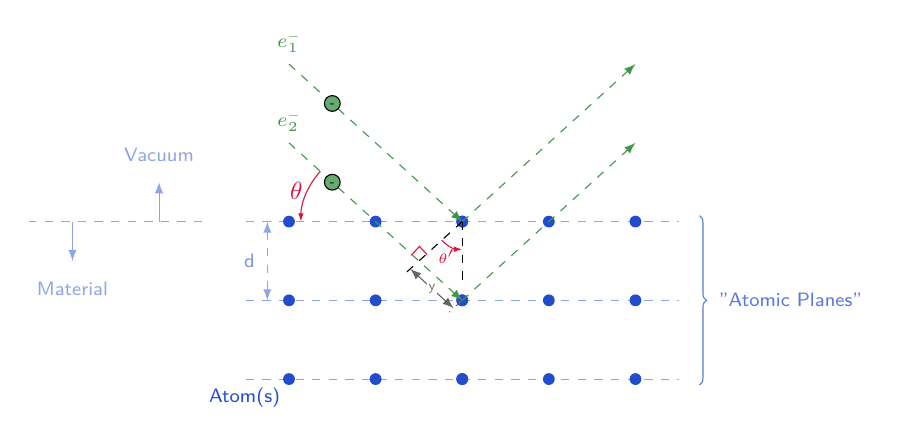
\begin{tikzpicture}[atomplane/.style={ScienceBlue!50,dashed,thin}]
		
		\def\dPlaneHeight{1}
		\def\PlaneWidth{5.5}
		
		\def\NumAtomstoDisplay{5}
		\def\AtomGap{\PlaneWidth/\NumAtomstoDisplay}
		
		
		
		\coordinate (P0Left) at (-\PlaneWidth/2,-\dPlaneHeight);
		\coordinate (P0Right) at (\PlaneWidth/2,-\dPlaneHeight);
		
		\coordinate (P1Left) at (-\PlaneWidth/2,0);
		\coordinate (P1Right) at (\PlaneWidth/2,0);
		
		\coordinate (P2Left) at (-\PlaneWidth/2,\dPlaneHeight);
		\coordinate (P2Right) at (\PlaneWidth/2,\dPlaneHeight);
		
		
		\draw[atomplane] (P2Left) -- (P2Right);
		\draw[atomplane] (P1Left) -- (P1Right);
		\draw[atomplane] (P0Left) -- (P0Right);
		
		\draw[atomplane,<->] ([shift={(0.1*\PlaneWidth/2,0)}]P2Left) -- node[ScienceBlue!60,left=1pt] {\scriptsize d} ([shift={(0.1*\PlaneWidth/2,0)}]P1Left);
		
		\foreach \atom in {0,1,2}{
			\fill[color=ScienceBlue] ({\atom*\AtomGap},-\dPlaneHeight) circle (0.075);
			\fill[color=ScienceBlue] ({-\atom*\AtomGap},-\dPlaneHeight) circle (0.075);
			
			\fill[color=ScienceBlue] ({\atom*\AtomGap},0) circle (0.075);
			\fill[color=ScienceBlue] ({-\atom*\AtomGap},0) circle (0.075);
			
			\fill[color=ScienceBlue] ({\atom*\AtomGap},\dPlaneHeight) circle (0.075);
			\fill[color=ScienceBlue] ({-\atom*\AtomGap},\dPlaneHeight) circle (0.075);
		}
		
		\node[inner sep=3,anchor=north east,ScienceBlue] at ({-\AtomGap*2},-\dPlaneHeight) {\scriptsize Atom(s)};
		
		
		\draw[decoration={brace,raise=7.5pt},color=ScienceBlue!75,decorate] (\PlaneWidth/2,\dPlaneHeight+0.075) -- node[color=ScienceBlue!75,right=11pt] {\scriptsize"Atomic Planes"} (\PlaneWidth/2,-\dPlaneHeight-0.075);
		
		
		\coordinate (MatLeft) at ({-(\PlaneWidth/2)-(0.5*\AtomGap)},\dPlaneHeight);
		\coordinate (MatRight) at ({-(\PlaneWidth/2)-(2.5*\AtomGap)},\dPlaneHeight);
		
		\coordinate (VacBot) at ({-(\PlaneWidth/2)-(1*\AtomGap)},\dPlaneHeight);
		\coordinate (VacTop) at ({-(\PlaneWidth/2)-(1*\AtomGap)},{\dPlaneHeight+(\dPlaneHeight*0.5)});
		
		\coordinate (MatTop) at ({-(\PlaneWidth/2)-(2*\AtomGap)},\dPlaneHeight);
		\coordinate (MatBot) at ({-(\PlaneWidth/2)-(2*\AtomGap)},{\dPlaneHeight-(\dPlaneHeight*0.5)});
		
		
		\draw[atomplane] (MatLeft) -- (MatRight);
		\draw[->,ScienceBlue!50] (VacBot) --(VacTop) node[color=ScienceBlue!50,above=4pt] {\scriptsize Vacuum};
		\draw[->,ScienceBlue!50] (MatTop) -- (MatBot) node[color=ScienceBlue!50,below=4pt] {\scriptsize Material};
		
		
		
		
		\coordinate (E1) at ({-2*\AtomGap},{3*\dPlaneHeight});
		\coordinate (E2) at ({-2*\AtomGap},{2*\dPlaneHeight});
		
		
		%% ELECTRON ONE
		\draw[->,dashed,ScienceGreen!75] (E1) node[color=ScienceGreen!75,above=0.5pt] {\scriptsize $e_1^-$} -- (0,\dPlaneHeight);
		\draw[fill=ScienceGreen!60] ({-1.5*\AtomGap},{2.5*\dPlaneHeight}) circle [radius = 0.1];
		\node[anchor=center] at ({-1.5*\AtomGap},{2.47*\dPlaneHeight}) {\tiny -};
		
		%% ELECTRON TWO
		\draw[->,dashed,ScienceGreen!75] (E2) node[color=ScienceGreen!75,above=0.5pt] {\scriptsize $e_2^-$} -- (0,0);
		\draw[fill=ScienceGreen!60] ({-1.5*\AtomGap},{1.5*\dPlaneHeight}) circle [radius = 0.1];
		\node[anchor=center] at ({-1.5*\AtomGap},{1.47*\dPlaneHeight}) {\tiny -};
		
		
		%% ANGLE OF INCIDENCE
		\coordinate (mid) at ({-1*\AtomGap},\dPlaneHeight);
		\coordinate (last) at ({-1.5*\AtomGap},\dPlaneHeight);
		\draw pic[mysmallarr,"\small $\theta$",ScienceRed,draw=ScienceRed,angle radius=27,angle eccentricity=1.14] {angle = E2--mid--last};
		
		
		
		\coordinate (E1end) at ({2*\AtomGap},{3*\dPlaneHeight});
		\coordinate (E2end) at ({2*\AtomGap},{2*\dPlaneHeight});
		
		\draw[->,dashed,ScienceGreen!75] (0,\dPlaneHeight) -- (E1end);
		\draw[->,dashed,ScienceGreen!75] (0,0) -- (E2end);
		
		
		
		%% RIGHT ANGLE AND THETA PRIME DEMONSTRATION
		\coordinate (A) at ({-\AtomGap},{\dPlaneHeight});
		\coordinate (B) at ({-0.5*\AtomGap},{0.485*\dPlaneHeight});
		\coordinate (C) at (0,\dPlaneHeight);
		\coordinate (D) at ($(E2)!(B)!(C)$);
			
		\draw[dashed] (0,\dPlaneHeight) -- (0,{0.25*\dPlaneHeight});
		\draw[dashed] (0,\dPlaneHeight) -- ({-0.7*\AtomGap},{0.3*\dPlaneHeight});
		
		\rightAngle{E2}{B}{C}{0.2}
		
		\coordinate (start2) at ({-0.7*\AtomGap},{0.3*\dPlaneHeight});
		\coordinate (mid2) at (0,\dPlaneHeight);
		\coordinate (last2) at (0,{0.25*\dPlaneHeight});
		\draw pic[mysmallarr,"\tiny $\theta'$",ScienceRed,draw=ScienceRed,angle radius=10,angle eccentricity=1.4] {angle = start2--mid2--last2};
		
		
		%% DISTANCE MEASUREMENT
		\draw[<->,black!60] ({-0.1*\AtomGap},{-0.1*\dPlaneHeight}) -- ({-0.6*\AtomGap},{0.4*\dPlaneHeight}) node[midway,fill=white,inner sep=0.5]{\tiny y};
		\draw[dashed,black!60] (0,0) -- ({-0.15*\AtomGap},{-0.15*\dPlaneHeight});
		
		
		
	\end{tikzpicture}
\end{document}